\section{Preliminary Sizing}

The first stage sized a solid-propellant antiship missile equivalent to the Exocet/MM40 class. The professor's sizing script was used as reference: atmospheric properties were computed at low altitude, drag was estimated at cruise, the booster accelerated the missile to cruise Mach number, and the sustainer was sized to balance cruise drag for the required range.

\subsection{Main Assumptions}

\begin{itemize}
    \item Cruise speed: Mach \(0.9\);
    \item Required range: \(70~\text{km}\);
    \item Reference diameter: \(0.35~\text{m}\);
    \item Solid booster plus solid sustainer;
    \item Sustainer thrust approximately equal to cruise drag.
\end{itemize}

\subsection{Sizing Results}

\begin{table}[H]
\centering
\caption{Final preliminary missile dimensions and masses.}
\begin{tabular}{lc}
\toprule
Parameter & Value \\
\midrule
Diameter & \(0.35~\text{m}\) \\
Total length & \(5.80~\text{m}\) \\
Launch mass & \(855~\text{kg}\) \\
Empty mass & \(508.20~\text{kg}\) \\
Total propellant mass & \(346.80~\text{kg}\) \\
Propellant fraction & \(40.6\%\) \\
Cruise speed & \(306.23~\text{m/s}\) \\
Simulated range & \(71.09~\text{km}\) \\
\bottomrule
\end{tabular}
\end{table}

\begin{table}[H]
\centering
\caption{Solid propulsion sizing.}
\begin{tabular}{lcc}
\toprule
Parameter & Booster & Sustainer \\
\midrule
Burn time & \(4.00~\text{s}\) & \(228.59~\text{s}\) \\
Mean thrust & \(65.46~\text{kN}\) & \(2.319~\text{kN}\) \\
Propellant mass & \(121.44~\text{kg}\) & \(225.36~\text{kg}\) \\
Grain length & \(1.047~\text{m}\) & \(2.286~\text{m}\) \\
Specific impulse & \(220~\text{s}\) & \(240~\text{s}\) \\
\bottomrule
\end{tabular}
\end{table}

\begin{figure}[H]
\centering
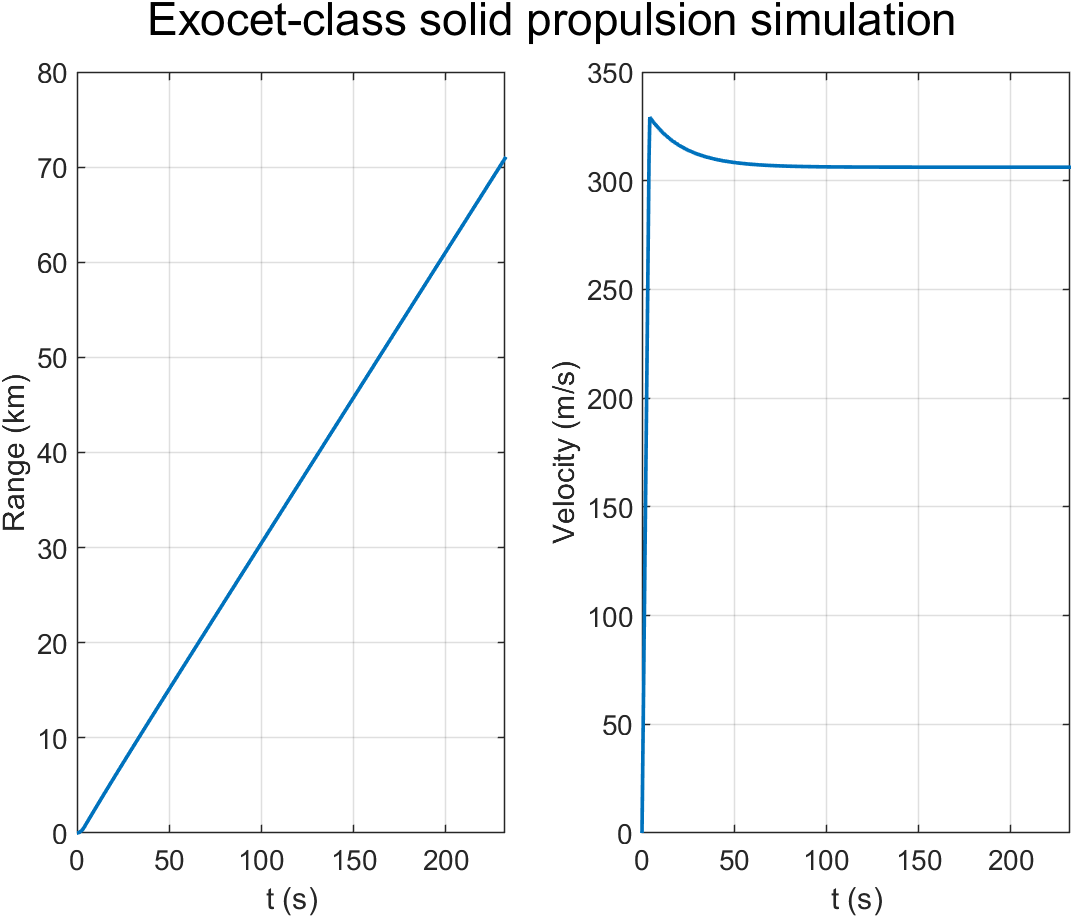
\includegraphics[width=0.88\textwidth]{figures/range_velocity.png}
\caption{Range and velocity from the preliminary propulsion simulation.}
\end{figure}

The sizing simulation reached \(71.09~\text{km}\), above the \(70~\text{km}\) requirement. This result became the basis for later mass, propulsion and geometry definitions.
